\subsection{Test of control region with isolated track in CR5}
\label{sec:CR5}

[NEED TO VERIFY THAT THE DESCRIPTION OF SCALE FACTORS IS CORRECT AND
ADD A LITTLE BIT OF DETAIL, AS NOTED IN THE TEXT]

This CR consists of events that pass all cuts but fail the isolated
track veto cut.  These events (especially in the tail of $M_T$) are 
predominantly $t\bar{t}$ dileptons.  Thus the test in this control
regions is similar to that performed in CR4 and described
in Section~\ref{sec:CR4-valid}.  There is some non-trivial 
complementarity because CR5 also includes events with 
taus and events with electrons or muons below the threshold of
the CR4 selection.  Also, this test is somewhat sensitive to
the simulation of the track isolation requirement, since the
number of dilepton events in CR5 depends on the (in)efficiency 
of that cut.



In CR5 there is also a significant component
of $t\bar{t} \to \ell +$ jets, where one of the jets fluctuates
to an isolated track.  This component dominates at low $M_T$
and is not necessarily well reproduced quantitatively by the 
simulation.  This makes the normalization of the top MC a little bit tricky.
We define a ``pre-veto'' sample as the sample of events that pass
all cuts without any isolated track requirements.  This sample is
dominated by $t\bar{t} \to \ell +$ jets.  We normalize the dilepton
component of the top MC to that sample (NEED TO EXPLAIN EXACTLY HOW).
Next we define a ``post-veto'' sample as the events that have an
isolated track.  The $t\bar{t} \to \ell +$ jets component is 
normalized in this sample (ALSO, NEED TO EXPLAIN HOW, EXACTLY).
These normalization factors are summarized in Table~\ref{tab:cr5mtsf}.

The underlying \met\ and $M_T$ distributions are shown in 
Figures~\ref{fig:cr5met} and~\ref{fig:cr5mtrest}.  The data-MC agreement
is quite good.  Quantitatively, this is also shown in Table~\ref{tab:cr5yields}.


\begin{table}[!h]
\begin{center}
\begin{tabular}{l||c|c|c|c}
\hline
Sample              & CR5A & CR5B & CR5C & CR5D \\
\hline
\hline
Muon pre-veto \mt-SF      & $0.98 \pm 0.02$ & $0.95 \pm 0.04$ & $0.99 \pm 0.08$ & $0.89 \pm 0.15$ \\
Muon post-veto \mt-SF     & $1.28 \pm 0.07$ & $1.20 \pm 0.13$ & $1.22 \pm 0.24$ & $1.25 \pm 0.43$ \\
\hline
\hline
Electron pre-veto \mt-SF          & $0.83 \pm 0.02$ & $0.75 \pm 0.04$ & $0.64 \pm 0.07$ & $0.63 \pm 0.12$ \\
Electron post-veto \mt-SF         & $1.10 \pm 0.08$ & $1.02 \pm 0.11$ & $0.89 \pm 0.19$ & $1.27 \pm 0.41$ \\
\hline
\end{tabular}
\caption{ \mt\ peak Data/MC scale factors. The pre-veto SFs are applied to the
  \ttdl\ sample, while the post-veto SFs are applied to the single
  lepton samples. The raw MC is used for backgrounds from rare processes.
  The uncertainties are statistical only.
\label{tab:cr5mtsf}}
\end{center}
\end{table}


\begin{table}[!h]
\begin{center}
\begin{tabular}{l||c|c|c|c}
\hline
Sample              & CR5A & CR5B & CR5C & CR5D \\
\hline
\hline
Muon MC                   & $293 \pm 9$ & $161 \pm 7$ & $51 \pm 4$ & $16 \pm 2$ \\
Muon Data                 & $315$ & $165$ & $62$ & $13$ \\
\hline
Muon Data/MC SF           & $1.07 \pm 0.07$ & $1.03 \pm 0.09$ & $1.21 \pm 0.18$ & $0.82 \pm 0.25$ \\
\hline
\hline
Electron MC               & $253 \pm 8$ & $126 \pm 5$ & $37 \pm 3$ & $12 \pm 2$ \\
Electron Data             & $286$ & $135$ & $39$ & $15$ \\
\hline
Electron Data/MC SF       & $1.13 \pm 0.08$ & $1.07 \pm 0.10$ & $1.07 \pm 0.19$ & $1.21 \pm 0.35$ \\
\hline
\end{tabular}
\caption{ Yields in \mt\ tail comparing the MC prediction (after
  applying SFs) to data. The uncertainties are statistical only.
\label{tab:cr5yields}}
\end{center}
\end{table}

\begin{figure}[hbt]
  \begin{center}
        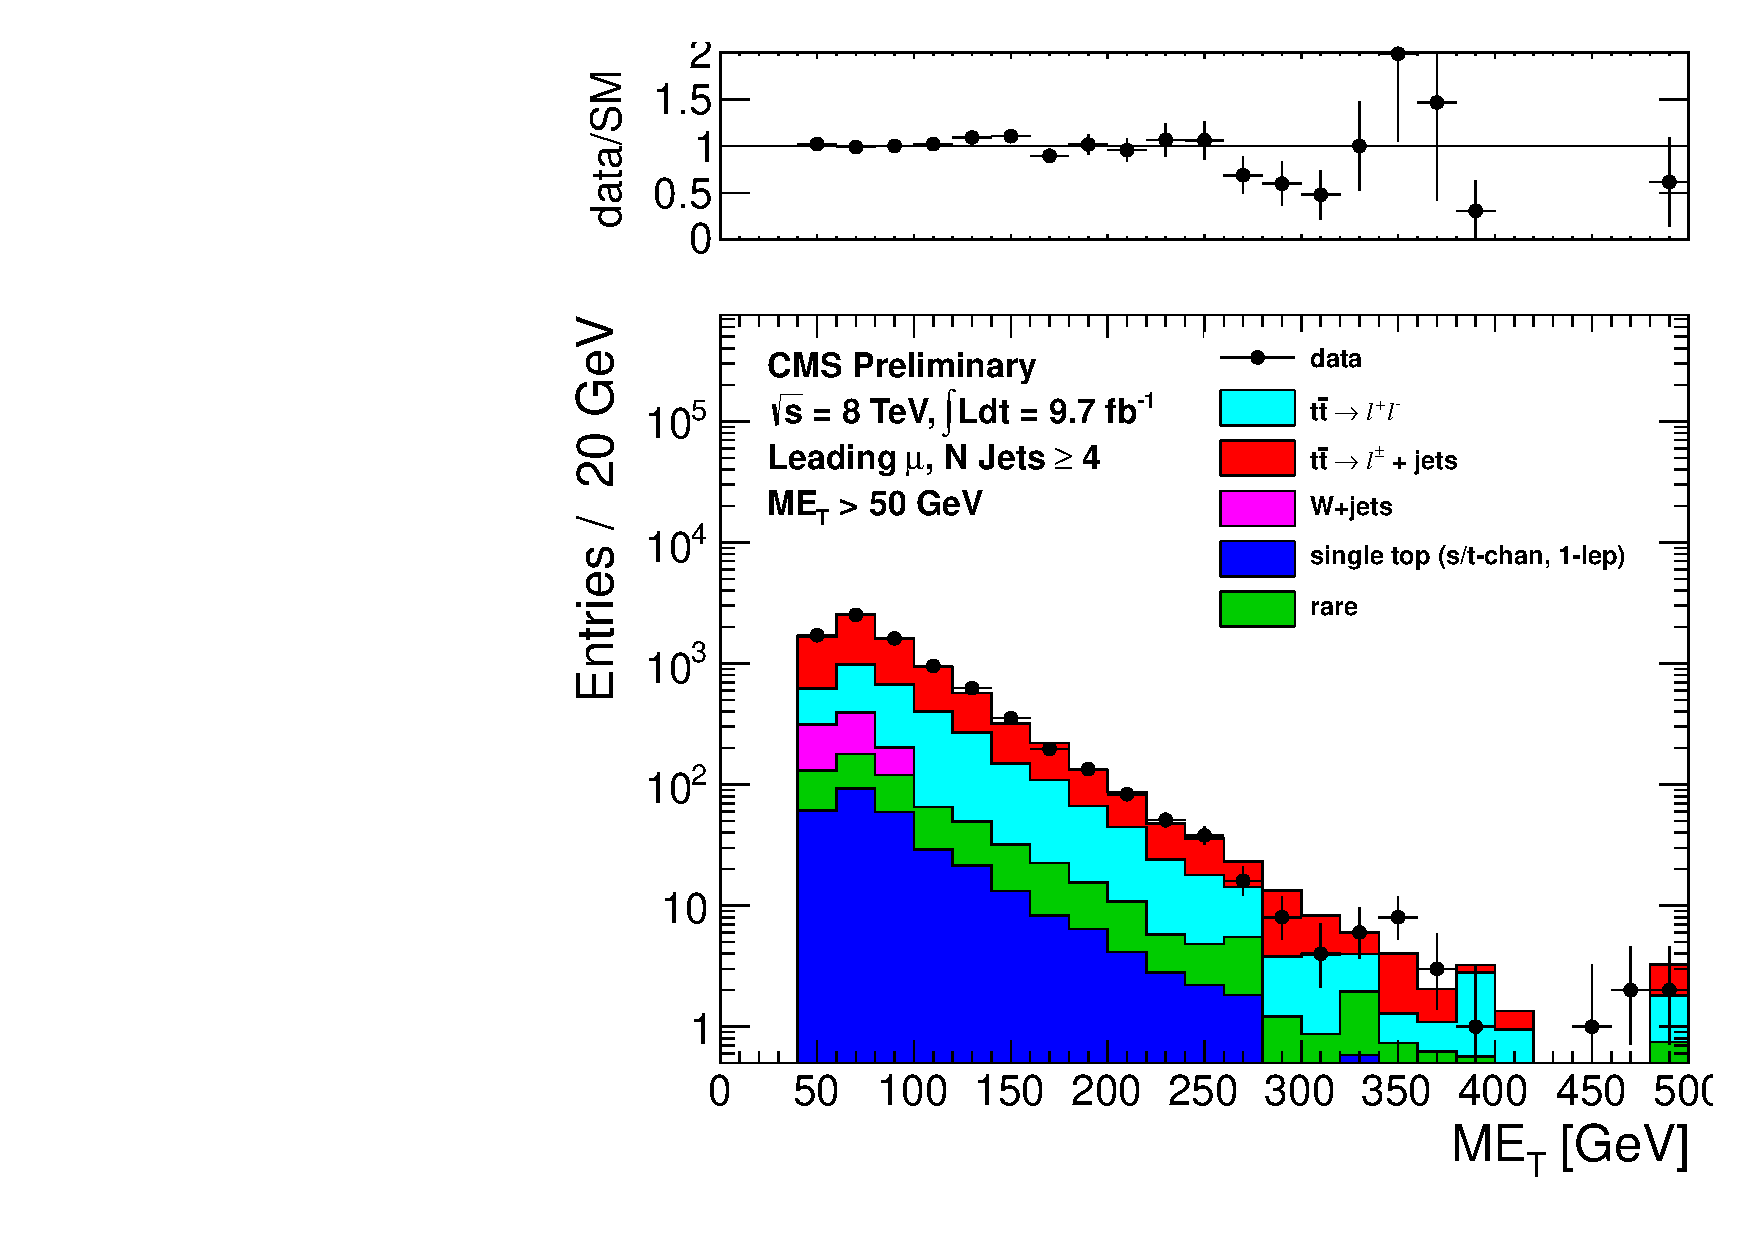
\includegraphics[width=0.5\linewidth]{plots/CR5plots/met_met50_leadmuo_nj4.pdf}%
        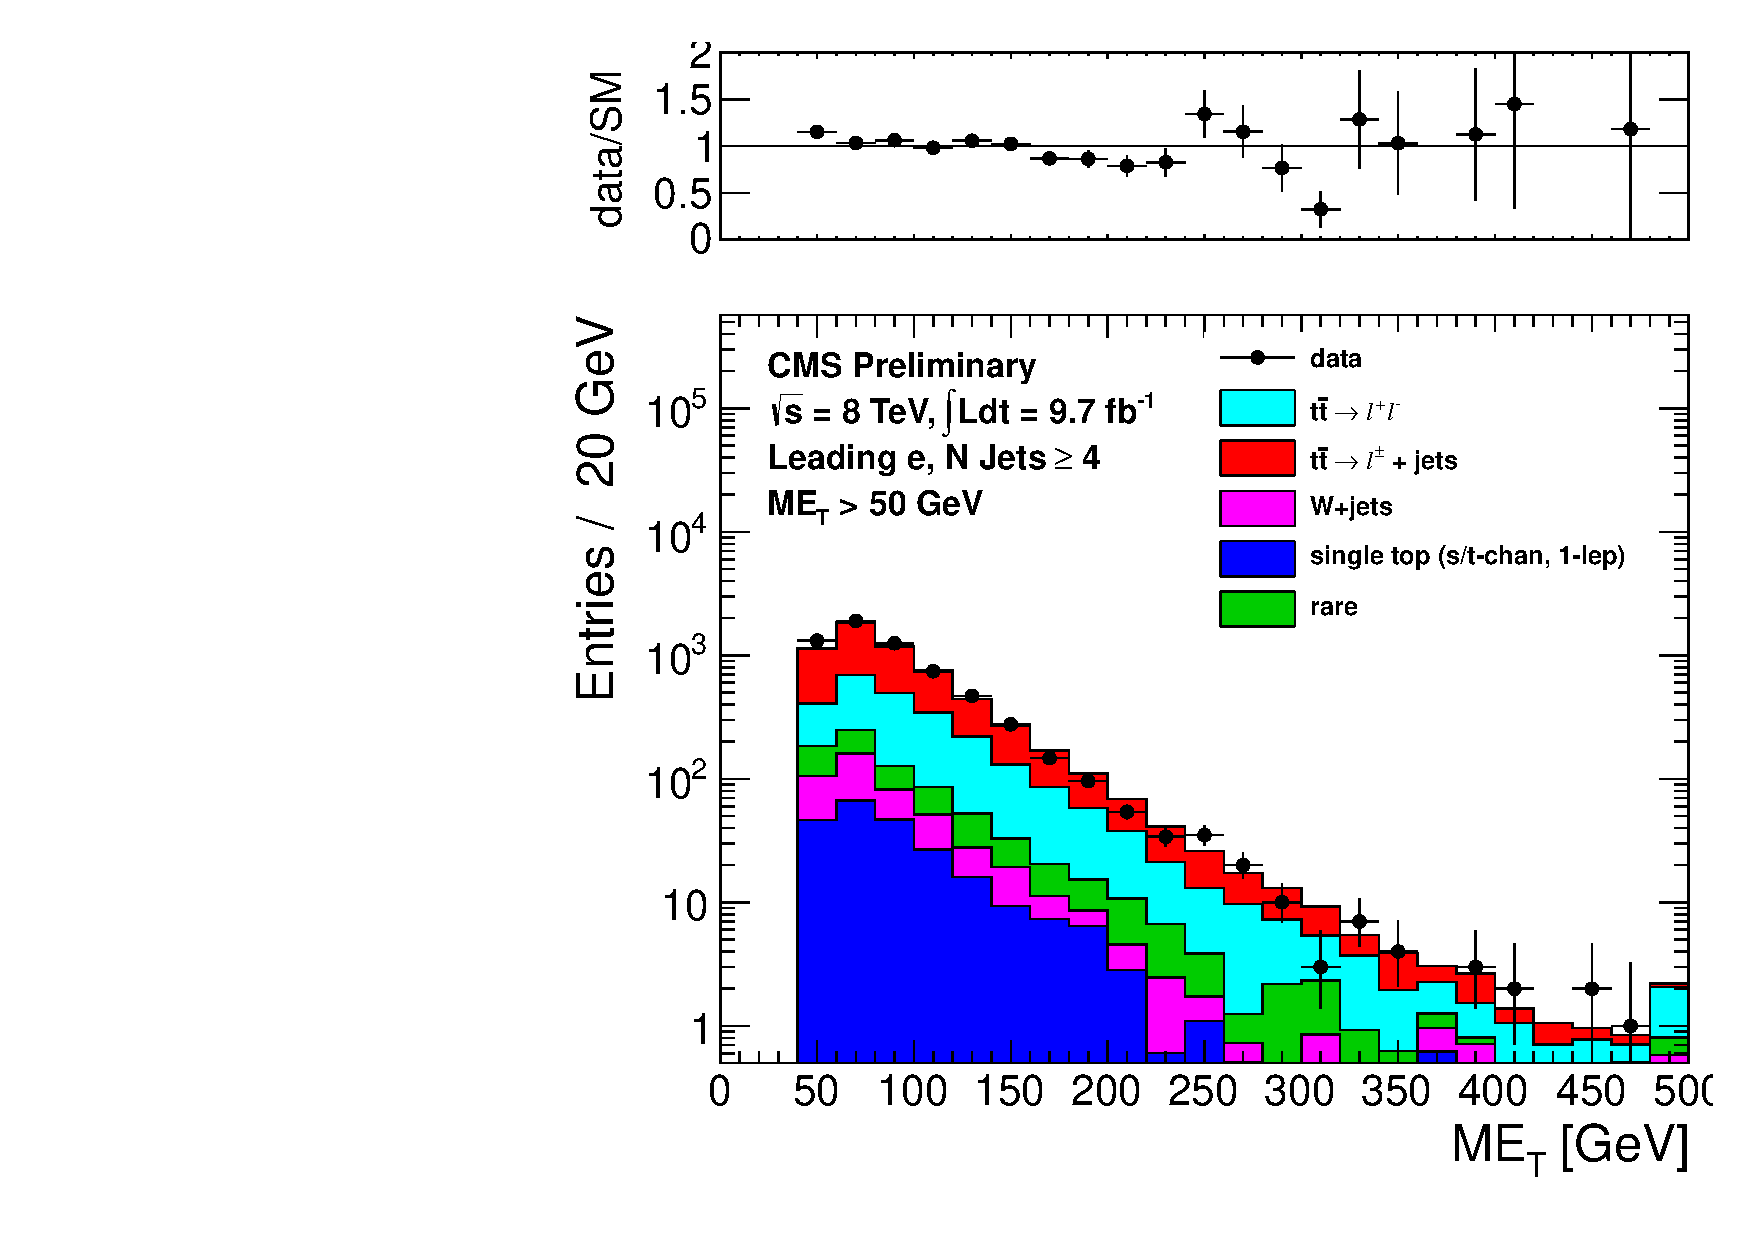
\includegraphics[width=0.5\linewidth]{plots/CR5plots/met_met50_leadele_nj4.pdf}
        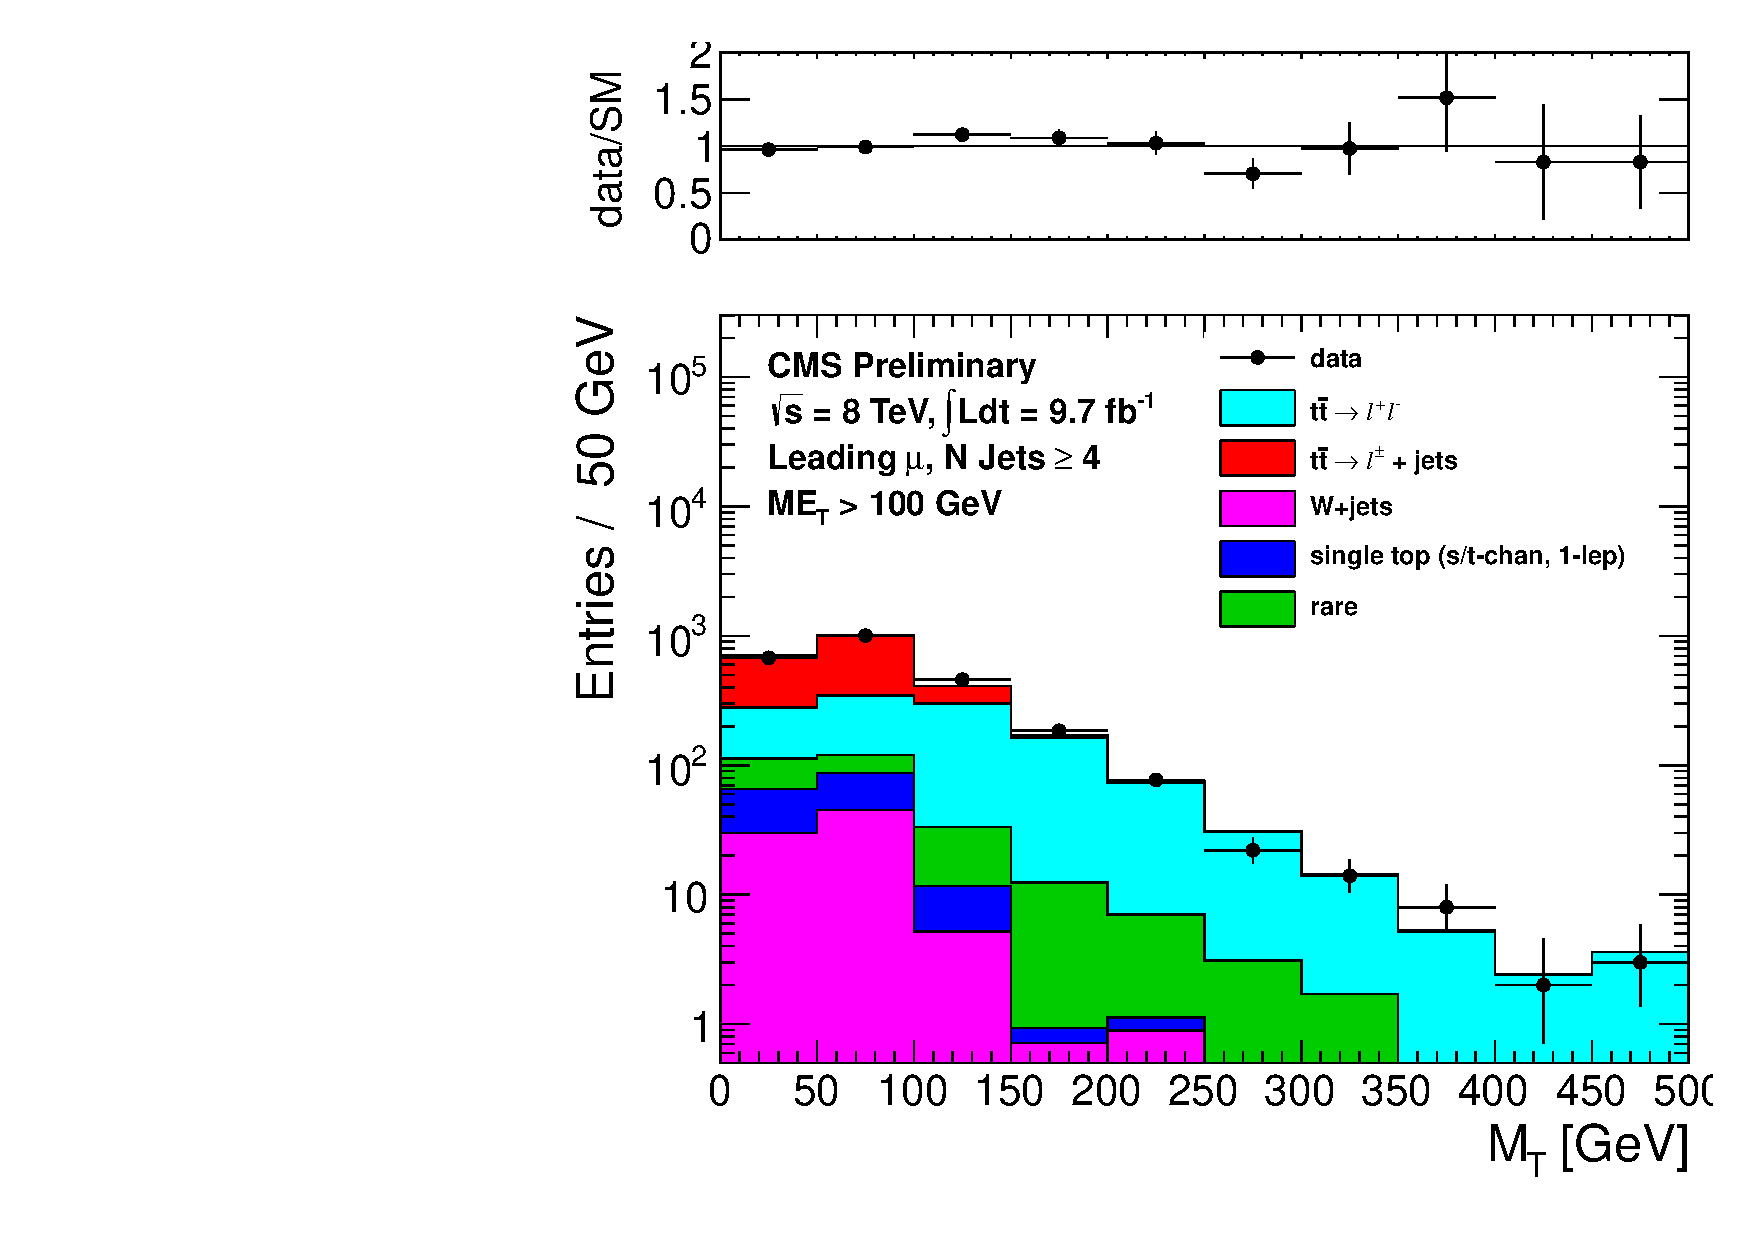
\includegraphics[width=0.5\linewidth]{plots/CR5plots/mt_met100_leadmuo_nj4.pdf}%
        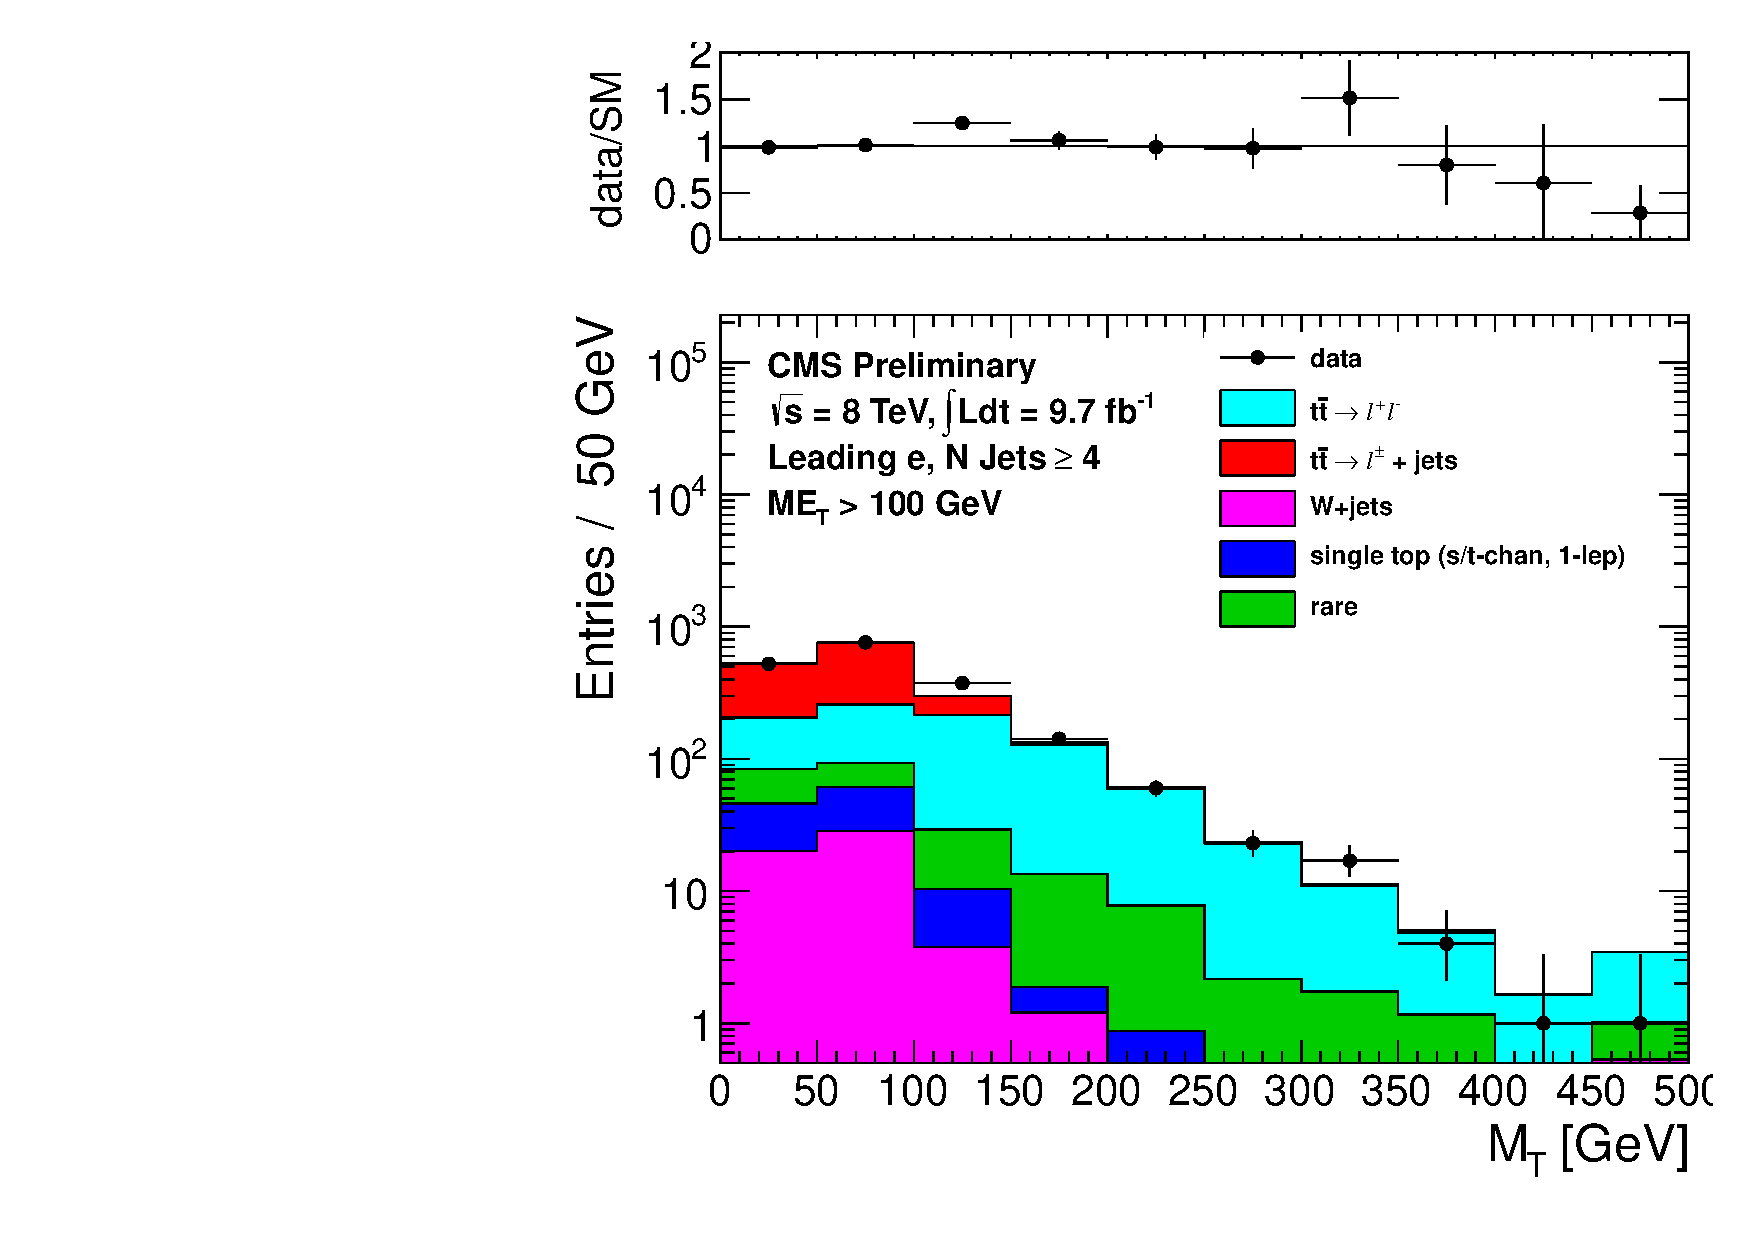
\includegraphics[width=0.5\linewidth]{plots/CR5plots/mt_met100_leadele_nj4.pdf}
    \caption{
      Comparison of the \met\ (top) and \mt\ for $\met>100$ (bottom) distributions in data vs. MC for events
      with a leading muon (left) and leading electron (right)
      satisfying the requirements of CR5. 
\label{fig:cr5met} 
}  
      \end{center}
\end{figure}

\begin{figure}[hbt]
  \begin{center}
        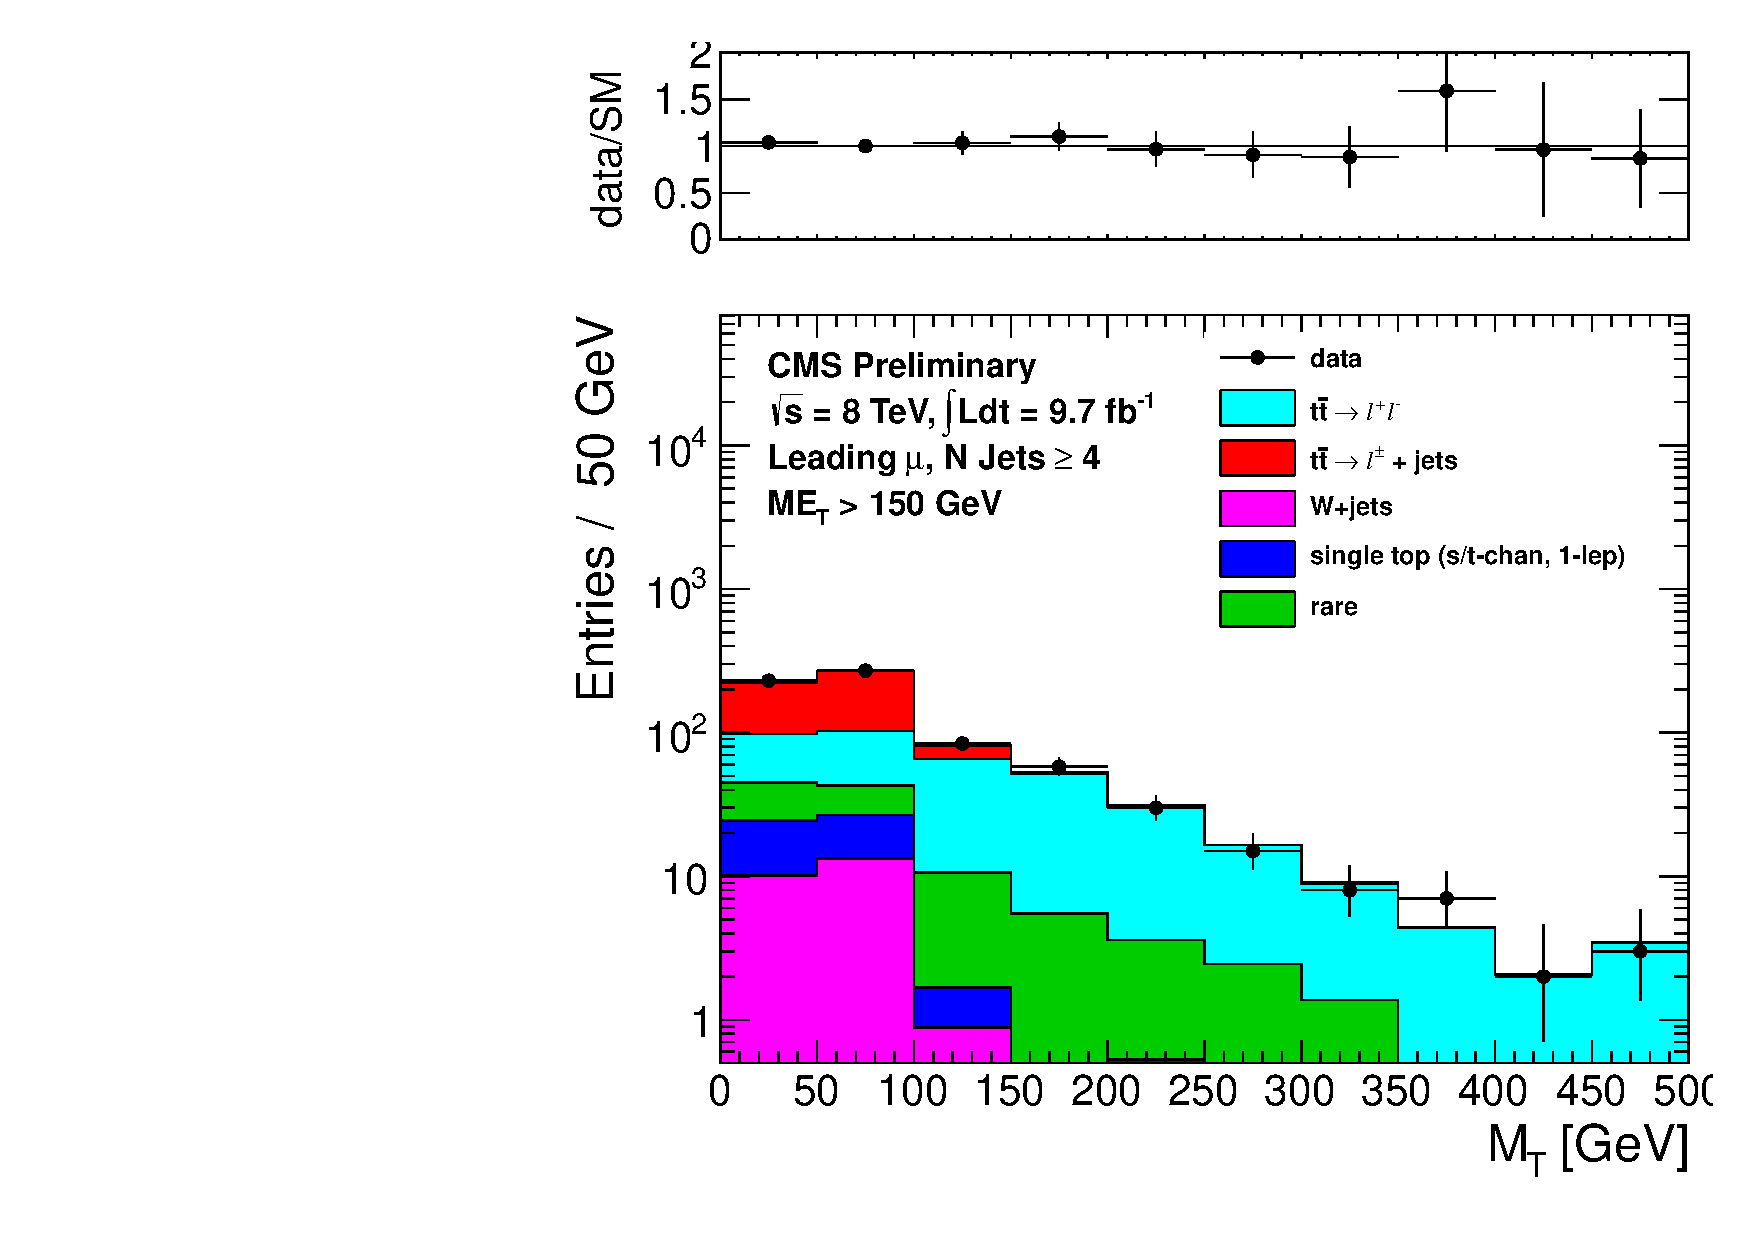
\includegraphics[width=0.5\linewidth]{plots/CR5plots/mt_met150_leadmuo_nj4.pdf}%
        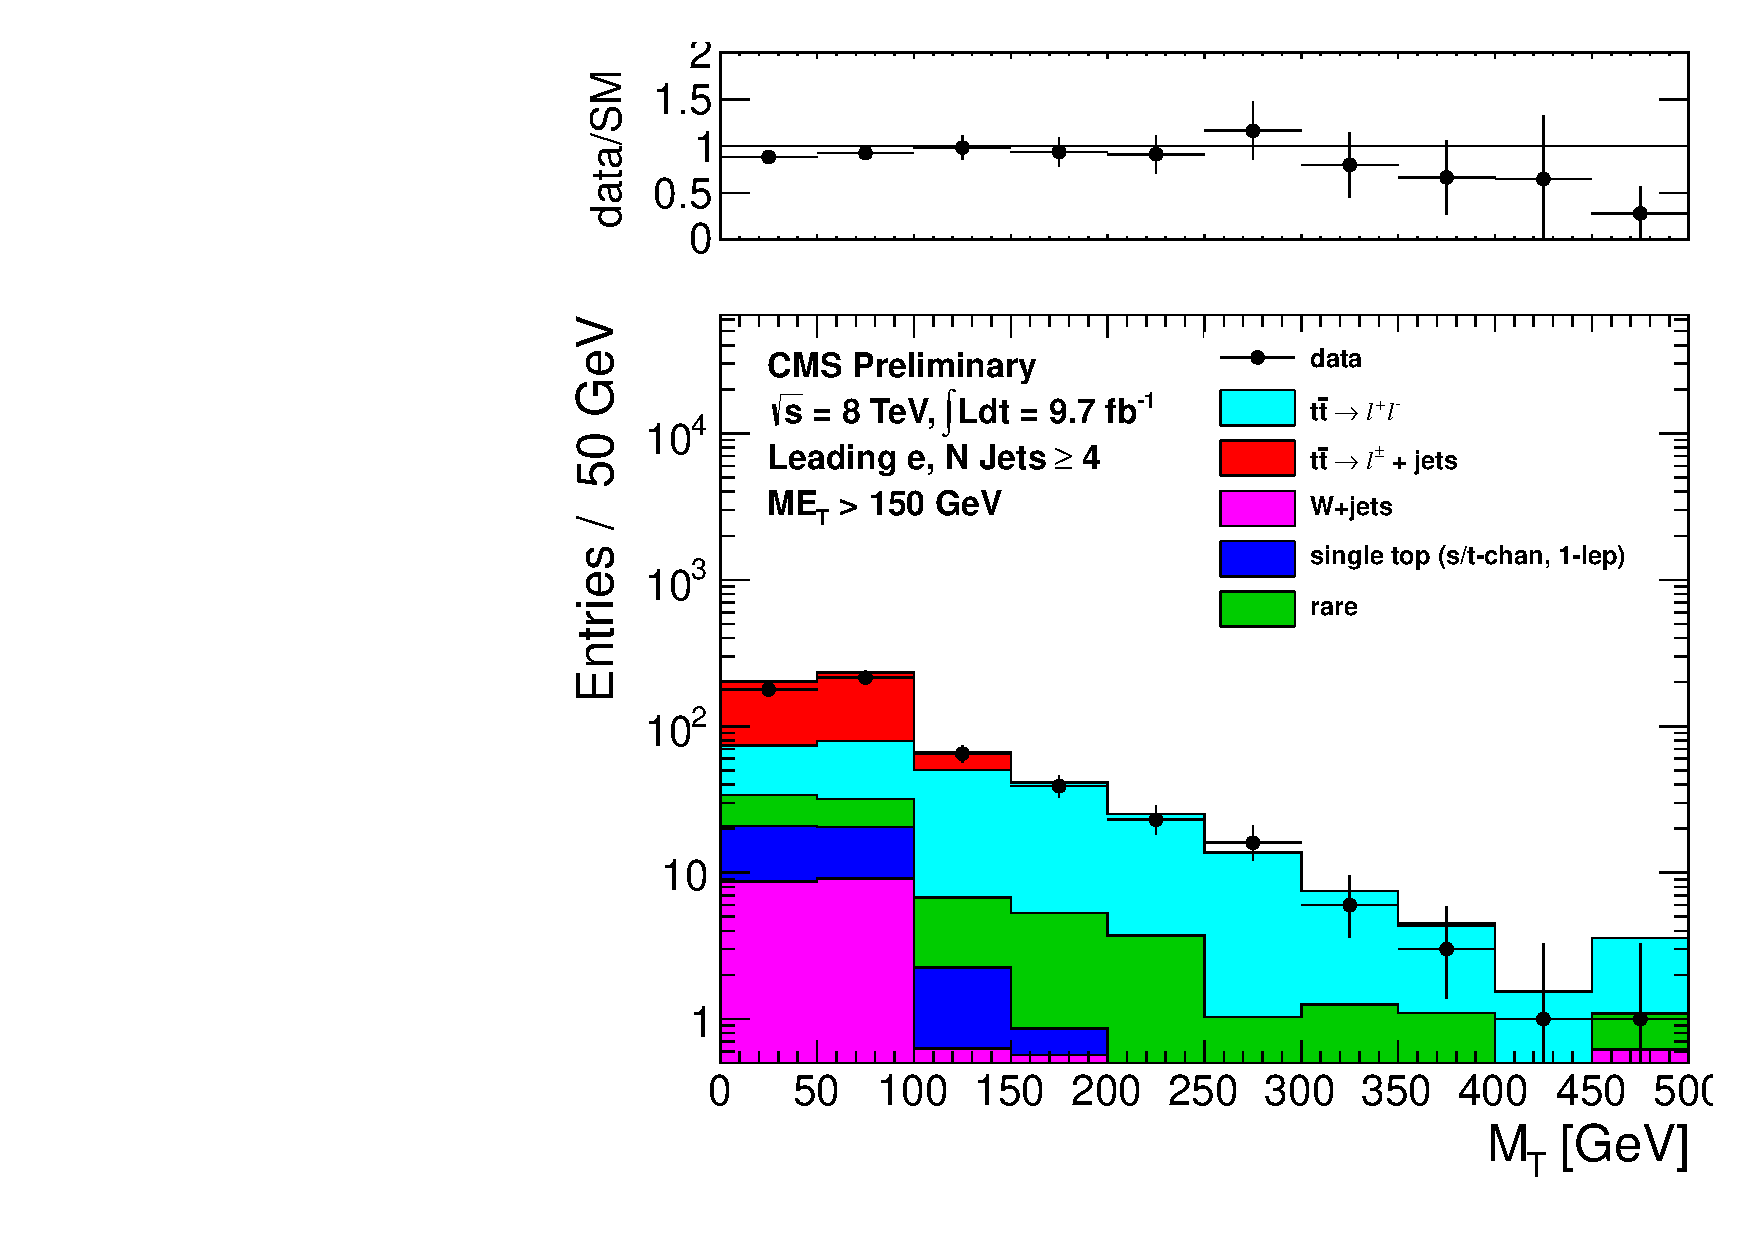
\includegraphics[width=0.5\linewidth]{plots/CR5plots/mt_met150_leadele_nj4.pdf}
        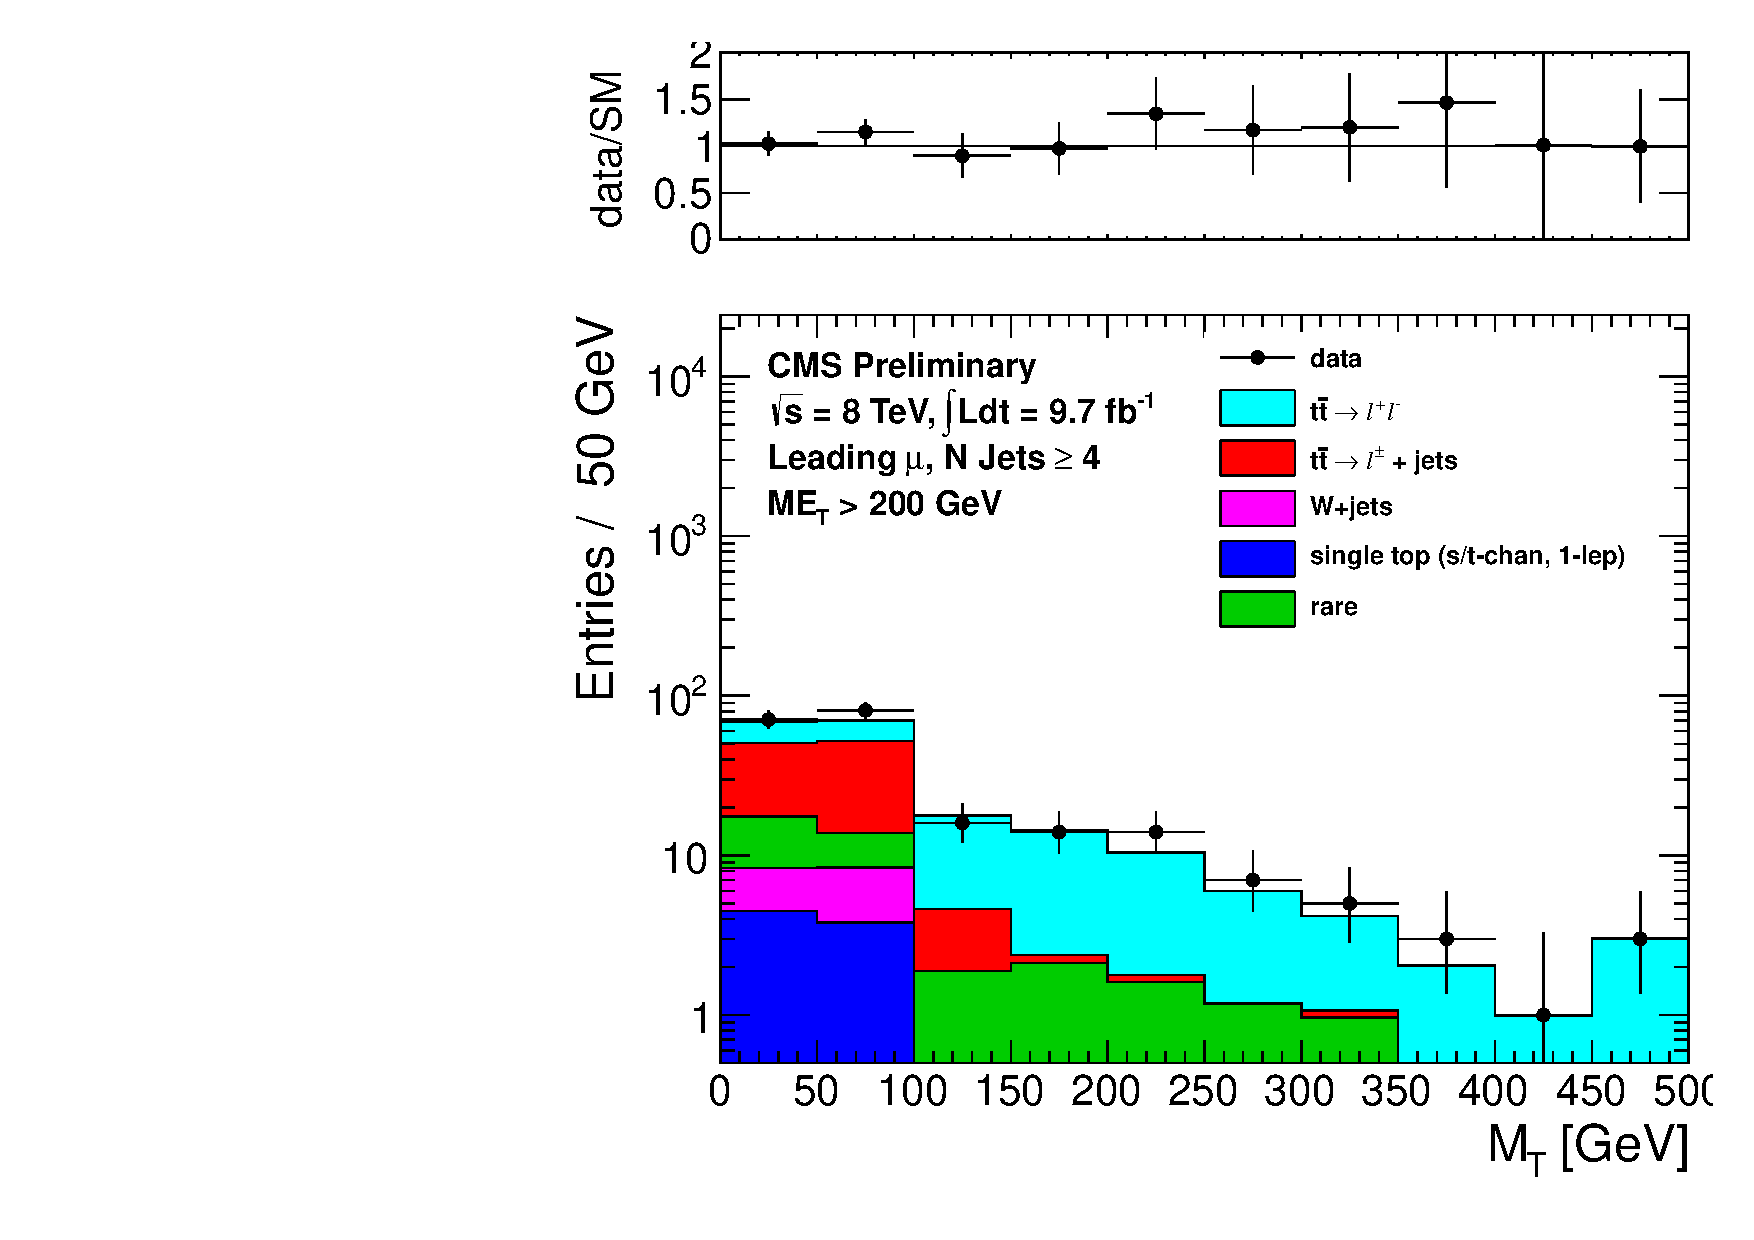
\includegraphics[width=0.5\linewidth]{plots/CR5plots/mt_met200_leadmuo_nj4.pdf}%
        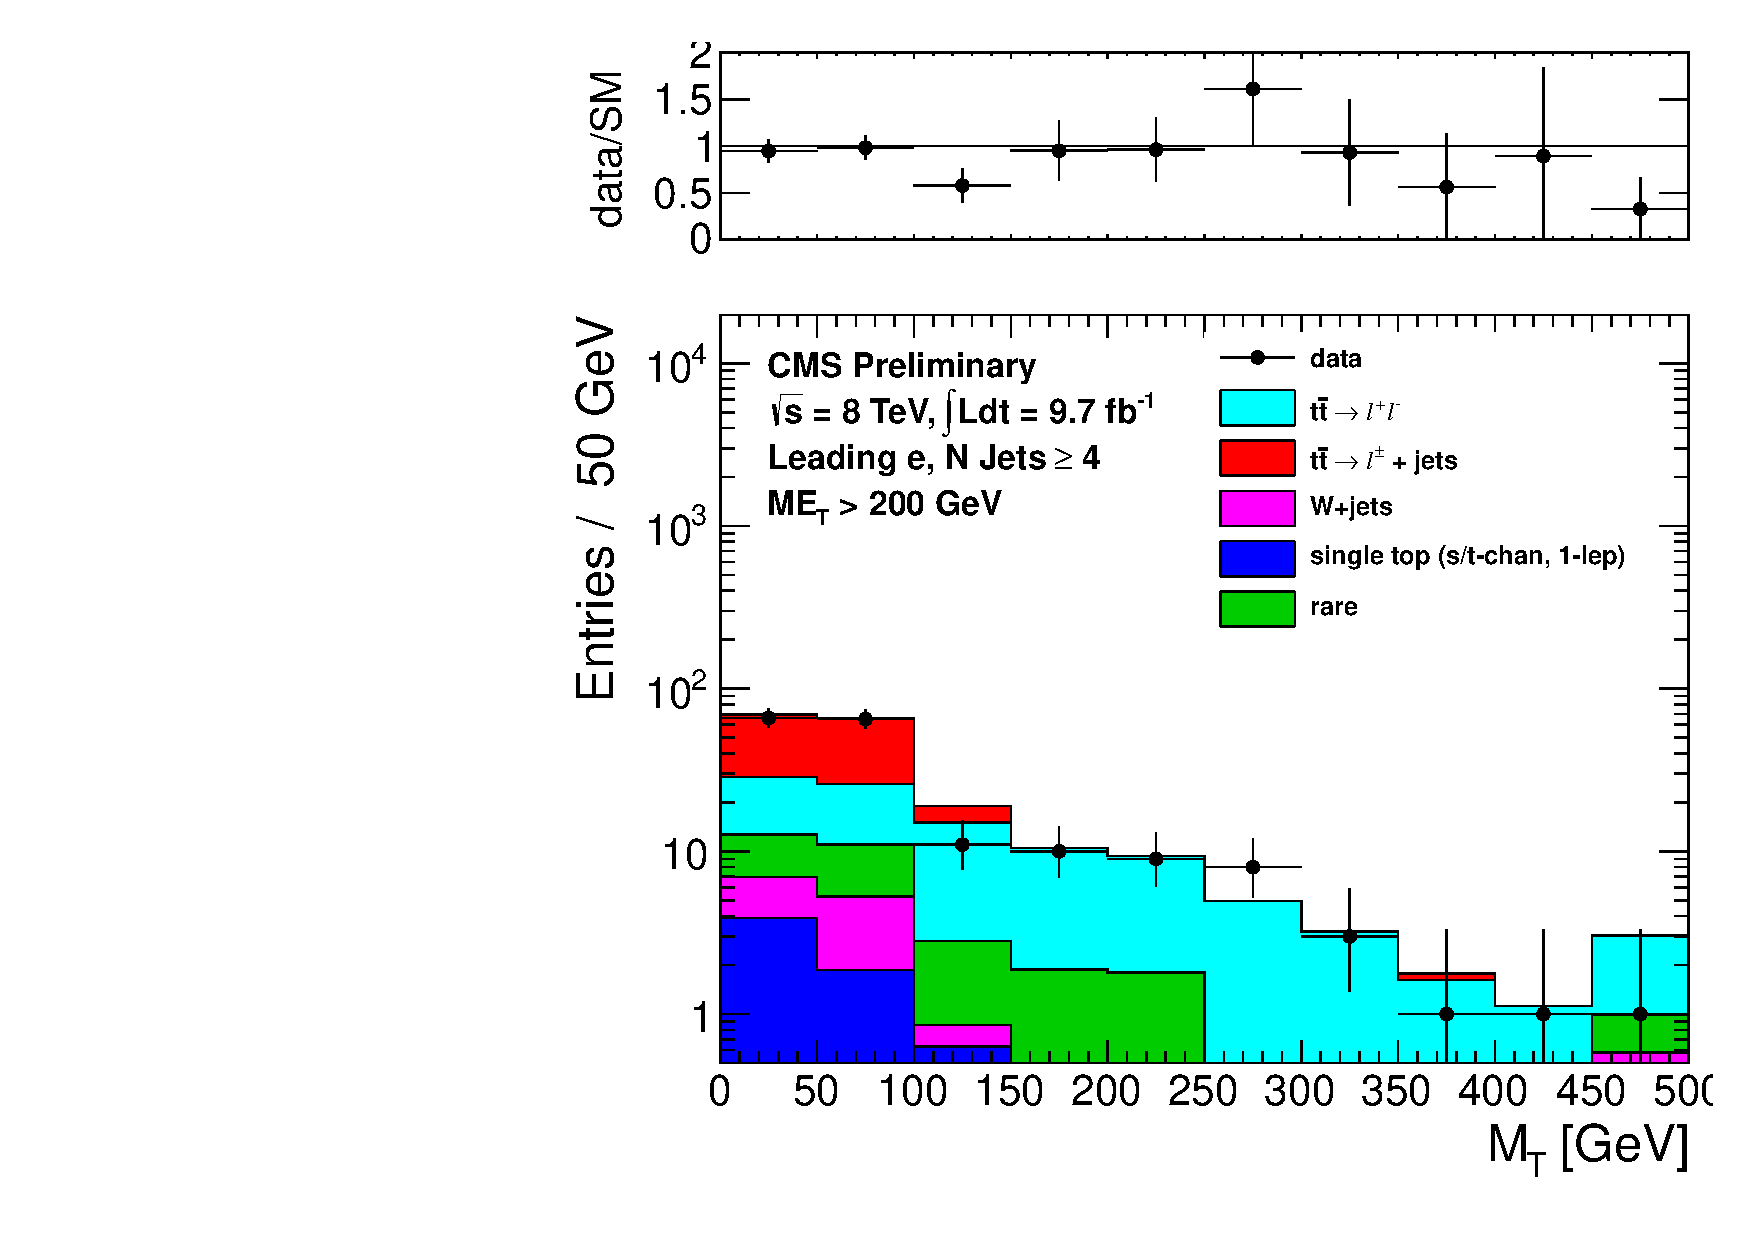
\includegraphics[width=0.5\linewidth]{plots/CR5plots/mt_met200_leadele_nj4.pdf}
        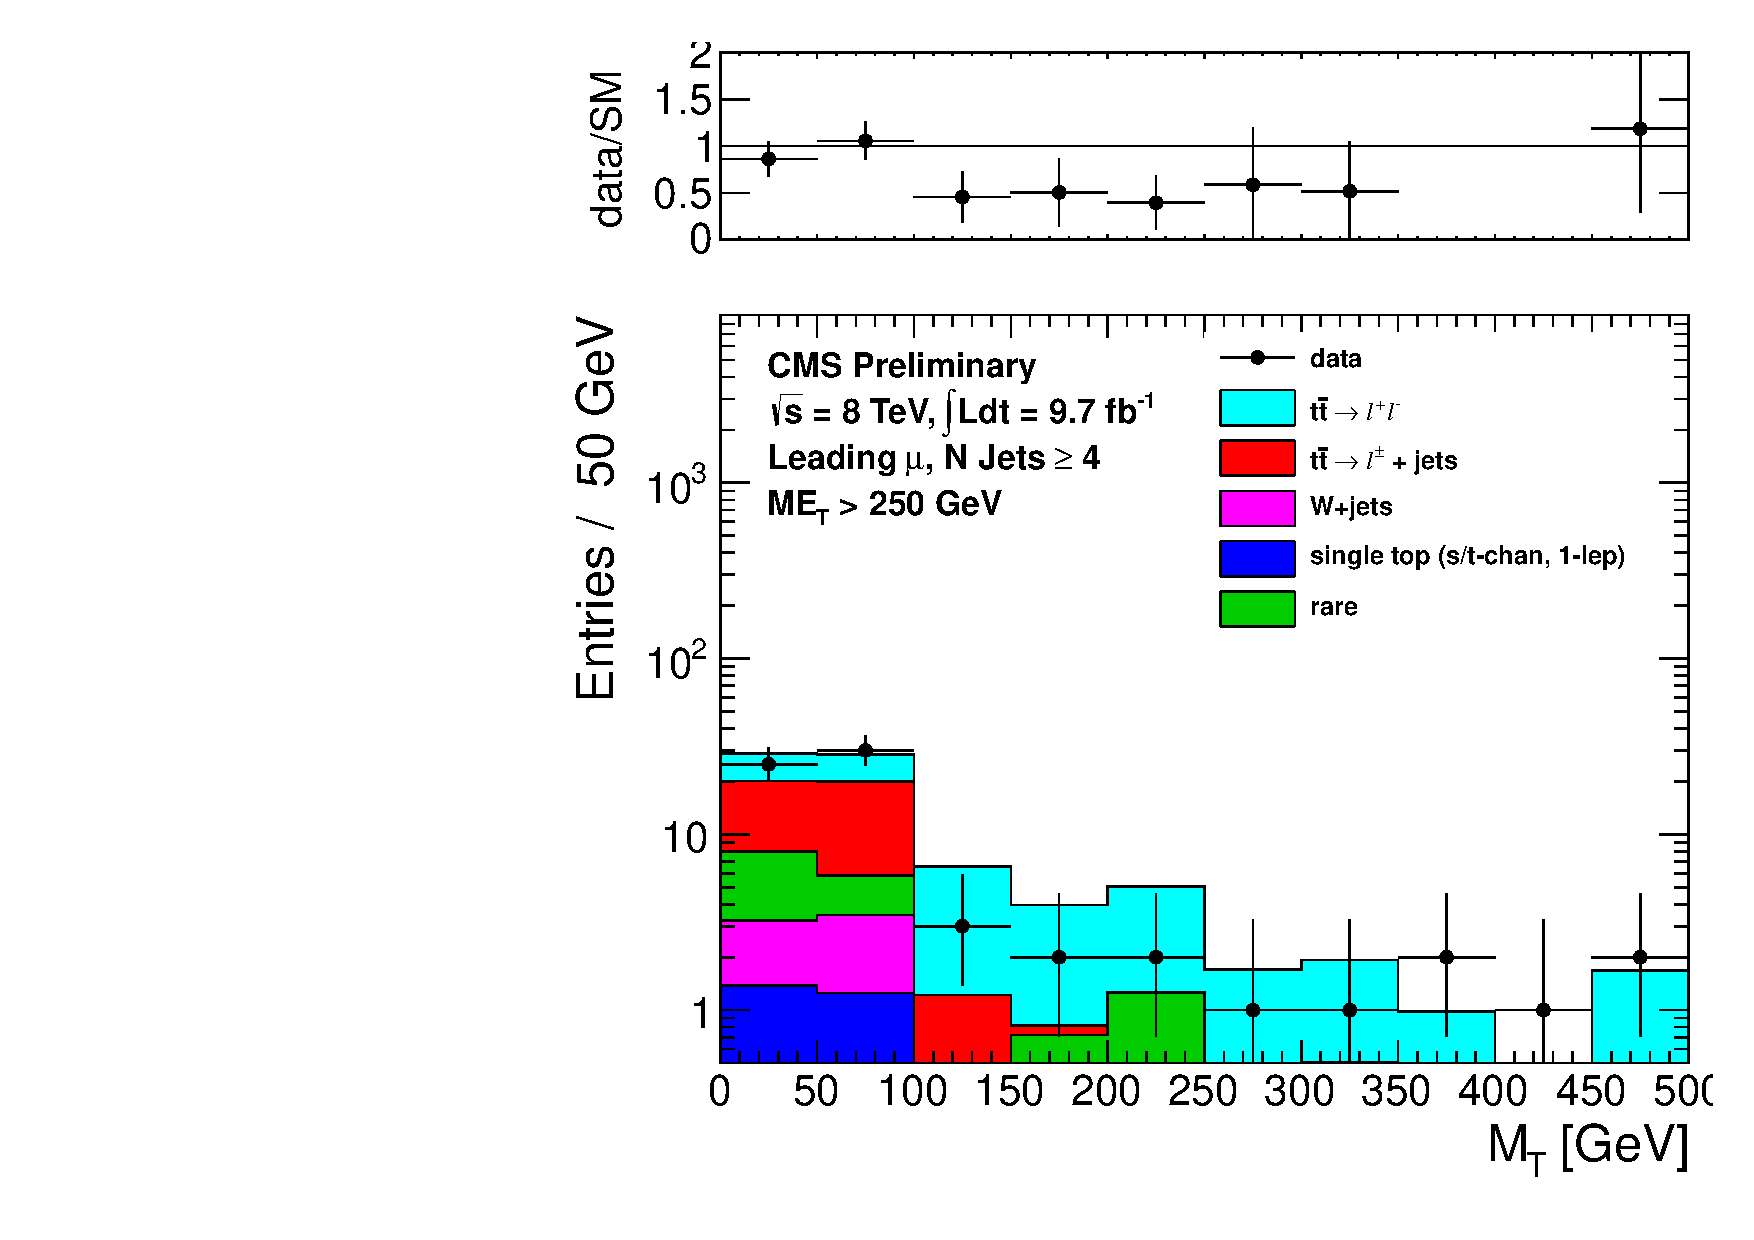
\includegraphics[width=0.5\linewidth]{plots/CR5plots/mt_met250_leadmuo_nj4.pdf}%
        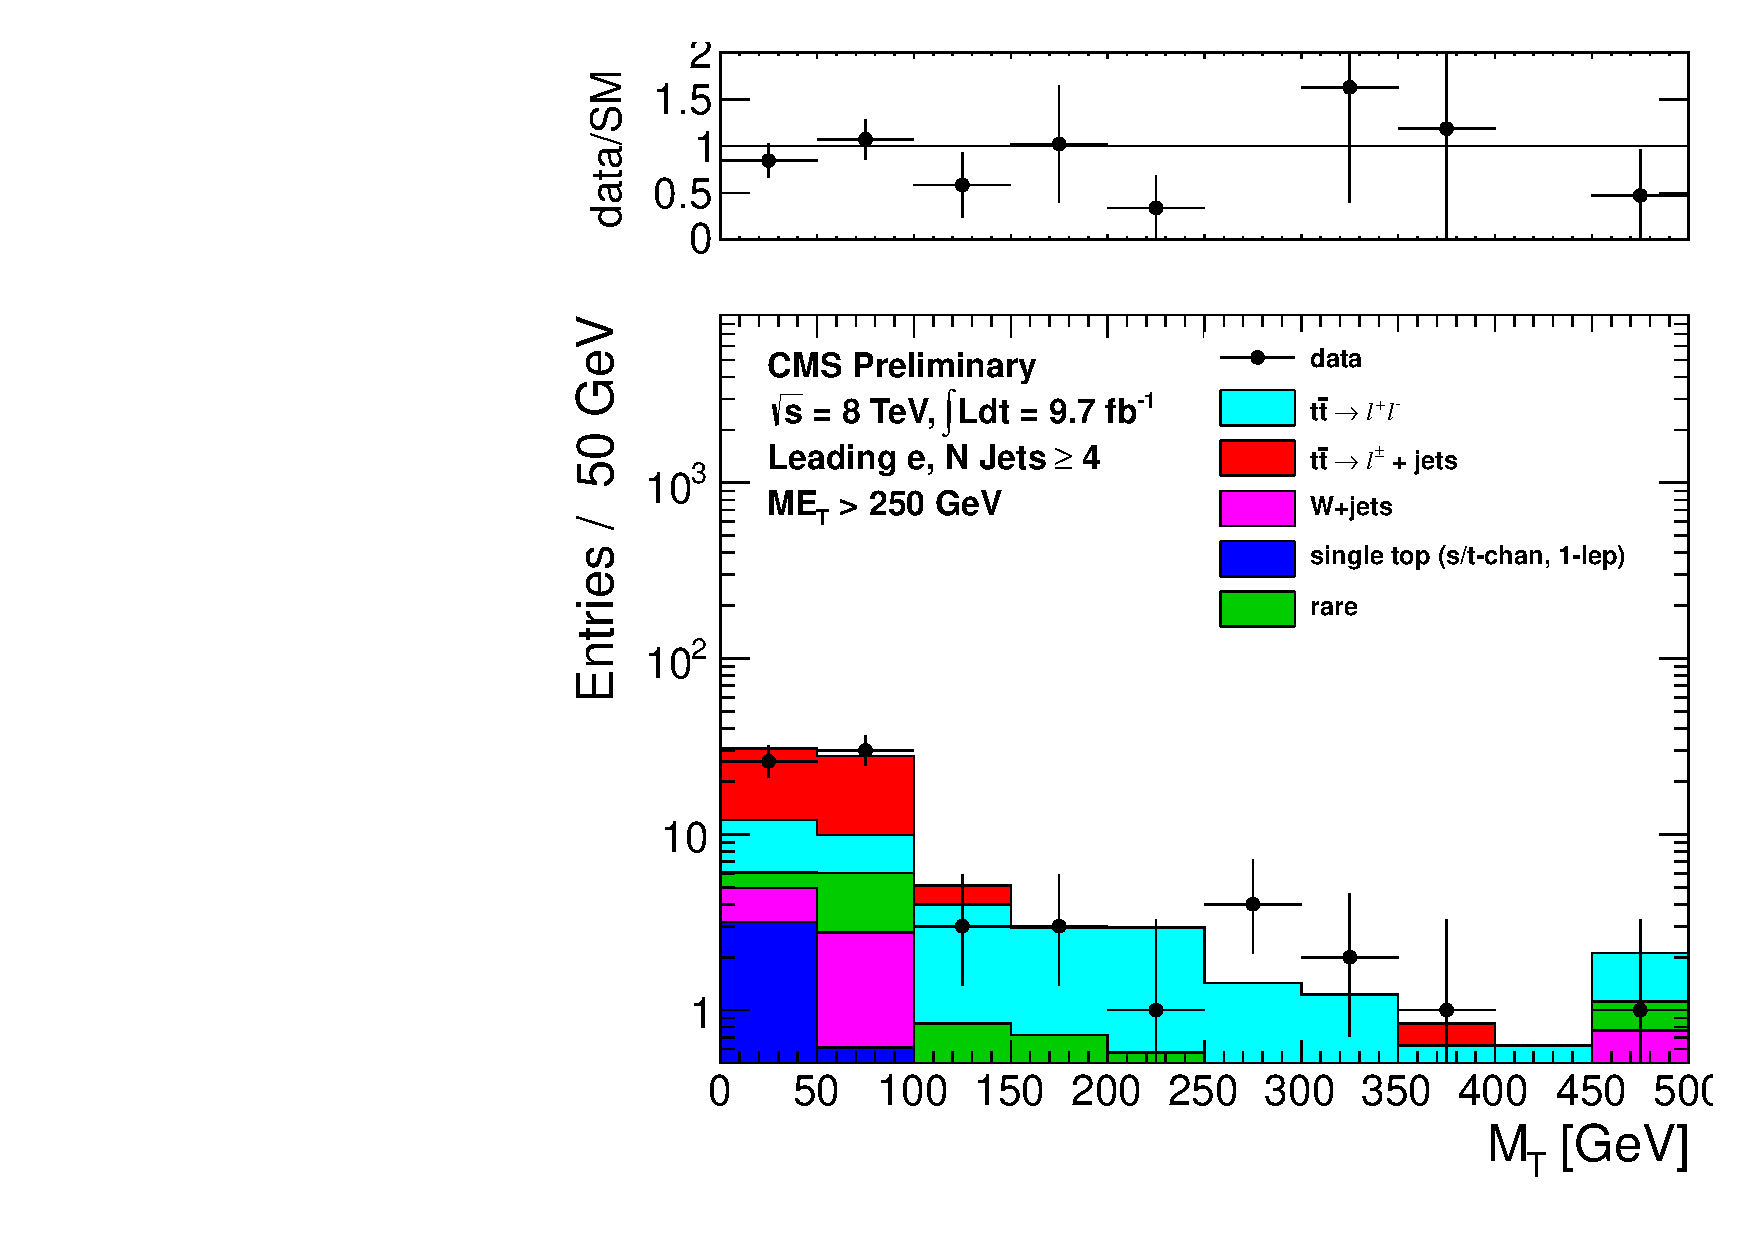
\includegraphics[width=0.5\linewidth]{plots/CR5plots/mt_met250_leadele_nj4.pdf}
    \caption{
      Comparison of the \mt\ distribution in data vs. MC for events
      with a leading muon (left) and leading electron (right)
      satisfying the requirements of CR5. The \met\ requirements used are
      150 GeV (top), 200 GeV (middle) and 250 GeV (bottom).
\label{fig:cr5mtrest} 
}  
      \end{center}
\end{figure}


\clearpage

